% 4-5 pages total.

% Goals:
% System architecture major design decisions and rationale.
% Implementation details (~1 page).
% Screenshots or other similar things (~1 page).
% Additional details; eg design diagrams in the Appendix.

% Marking:
% Is the software product well-designed, functional, reliable, robust, efficient, usable, maintainable, and well-documented? Has it been demonstrated?
% A-band: The software product is extremely well designed, implemented, and documented.

\chapter{Design \& Implementation}\label{design_implementation}

\section{System Foundations \& Application Flow}

A 2D image produced by the Cycles rendering engine can be considered a composite of multiple ``lighting passes''.
According to scene geometry, light sources and surface materials, the engine must compute the effects of direct/indirect diffuse light, direct/indirect specular light, shadow etc.
Similarly, ``data passes'' capture surface normals, depth information, and UV texture-coordinates.
Lighting and data passes can themselves be expressed as images and written to disk.
The typical use-case for this functionality is post-processing of render scenes, where compositing software is used to combine passes in different ways to affect characteristics of the final rendering.

For this project however, selected render passes are post-processed directly with Python, and used to inform placement of strokes through a combination of image-space processing and stroke-based rendering techniques. As such, the System builds directly on render passes produced by the Cycles engine in Blender, and these images form the fundamental input to the System. The combination of all strokes is rendered to an SVG image, which is the sole System output.

This high-level application flow is presented in Appendix \ref{appendix_design}, Figure \ref{flow}.

\section{Platform Considerations \& System Architecture}
% - Design for blender plugin (multifile).
% - Separation of blender-specific from backend.
% - Design considerations for testing (brief, cover testing in next section).
% - Levels of abstraction between modules.

Blender ships with an embedded Python interpreter\footnote{\url{https://docs.blender.org/api/2.79/info_overview.html}}, allowing arbitrary scripts to be executed within the Blender environment.
Blender's powerful Python API\footnote{\url{https://docs.blender.org/api/2.79/}} (specifically the \texttt{bpy} module), exposes session/scene data, allows automation of built-in functionality, and enables creation of UI elements.

Trivial scripts can be pasted into and executed from the built-in Python shell or editor, however good practice\footnote{\url{https://docs.blender.org/api/2.79/info_overview.html#script-loading}} dictates that more complex systems be encapsulated as a multi-file package{\footnote{\url{https://blender.stackexchange.com/questions/44532/best-practice-for-add-on-generation-with-many-functions-single-file-or-split-it}}.
To encourage distribution of useful modules, Blender provides a convenient ``add-on'' subsystem, which allows packages to be easily installed and toggled via the GUI.

An add-on is essentially a regular Python package, with two key additional requirements. 
The top-level package \texttt{\_\_init\_\_.py} must contain package metadata\footnote{\url{https://wiki.blender.org/wiki/Process/Addons/Guidelines/metainfo}}, and must implement \texttt{register()} and \texttt{unregister()} methods.
These methods allow the add-on subsystem to toggle visibility of contained classes within the Blender environment.

Beyond these simple requirements, no constraints are placed on compatible system architectures. 
Dependence on the \texttt{bpy} module however has practical implications for design and development.
\texttt{bpy} is shipped built-in to the embedded environment, and is not accessible outside of a running Blender session\footnote{At least not without complex and poorly documented workarounds: \url{https://blender.stackexchange.com/questions/102933/a-working-guidance-for-building-blender-as-bpy-python-module}}.
Indeed, the role of \texttt{bpy} is to query and alter the internal state of a Blender session, and has no functional use outside of this session (as would be the case when developing code in an IDE operating in a virtual environment).

This is generally not a concern for trivial systems where development and testing can be performed within Blender's simple script editor.
Due to the anticipated complexity of this System however, the power of an IDE was preferred (specifically debugging and re-factoring capabilities).

As such, a design decision was taken to de-couple \texttt{bpy} from as much of the application code as possible.
This was achieved by implementing a Model-View-Controller arrangement, presented in Appendix \ref{appendix_design}, Figure \ref{arch}.
The \texttt{view-controller} contains code with dependencies on \texttt{bpy}, which must run/tested within the clunky Blender environment. 
The \texttt{model} is free of \texttt{bpy} dependencies, and is run/tested in an IDE and virtual environment. 
The majority of application code - including all image processing logic and SVG rendering - is contained in the \texttt{model} which has no knowledge of the \texttt{view-controller}, or the wider Blender environment.

This design enabled the majority of development to take place outside of Blender.
Core rendering functionality provided by the \texttt{model} can be run directly, and strong de-coupling enables the backend \texttt{model} to be used with 3D modelling packages other than Blender, provided the necessary input render pass data can be made available on disk.

Some practical testing implications of this approach are discussed further in Section \ref{}.

\section{Domain Design}

The domain model is presented in Appendix \ref{appendix_design}, Figure \ref{domain}.

\subsection{View-Controller}

Code in this package is limited to essential add-on plumbing; GUI creation; manipulation of User-space settings within Blender; and triggering of \texttt{model} code.

Package structure is based upon existing well-known examples of Blender add-ons\footnote{Cycles, Archimesh}.

\subsection{Model}

A tiered approach is taken within this package, with each tier representing a distinct level of abstraction.

The \texttt{Illustrator} is the entry-point to the \texttt{model}. 
It is responsible for preparing all input data (reading render passes from disk), and triggering the necessary \texttt{elements} as required by User settings.
Classes in \texttt{elements} contain high-level logic required to create different art elements, namely \texttt{Silhouette}, \texttt{InternalEdges}, \texttt{Streamlines}, and \texttt{Stipples}.
In turn, \texttt{elements} rely upon classes in \texttt{primitives}, which provide universally useful functionality, such as modelling of \texttt{Path}s and creation of SVG \texttt{CurvedStroke}s.

\section{Implementation Details}

\subsection{Continuous Strokes \& Path Tracing}

The ultimate goal is to visualise an object (the render subject) as series of natural-looking SVG elements.
For ``continuous'' lines such as silhouettes, internal edges and streamlines, the SVG elements should also be continuous and smooth.
Bezier curves are supported by the SVG 1.1 specification, and can be rendered as continuous, smooth curves using composite curve-fitting\footnote{\url{https://gist.github.com/gumblex/047abdd163c3a3c96b64}} techniques.

To define such a curve, we need a notion of where each stroke should start, end, and through which points it should pass.
However, in this case, the input data is a series of raster images.
There is no notion of which pixels represent the start or end of a distinct stroke, or indeed any immediate way to identify the \emph{ordered sequence} of image-space coordinates which lie on the path between these points. A further problem is identifying the basic features themselves - for example which pixels represent a Silhouette, or Internal Edge? The implemented solution differs depending on context, however the main techniques are as follows.

\texttt{Silhouette} processes the object index pass with \texttt{skimage.measure.find\_contours}.
The object index map is a binary image, so by choosing an intensity value close to the maximum image intensity we are able to extract a closed-sequence of image-space coordinates which directly represent the Silhouette of the render subject.
This alone is not adequate.
If curve fitting is performed directly on this closed-loop, sharp corners would be likely be rounded, losing the character of the outline.
As such, an additional step is taken where sharp corners are detected using the Harris algorithm provided by \texttt{skimage}.
The continuous outline path is then split at each identified corner. Individual paths are then curve-fitted, allowing the outline to be correctly expressed.
This process is outlined graphically in Appendix \ref{impl_silhouette}.

No render pass directly indicates internal edges so a different approach is taken here, as outlined in Appendix \ref{impl_internal}.
Distinct internal edges are first detected and labelled using \texttt{skimage.feature.canny} and \texttt{skimage.measure.label}. Reusing \texttt{find\_contours} would not be appropriate here, as this would have the effect of detecting paths \emph{around} each edge line.
Instead, the end-point coordinates of each line are first detected.
The premise is that if a pixel only has one neighbouring occupied pixel in its Moore's neighbourhood, then it can be considered an end-point of the line.
End-points are computed efficiently for each line using convolution and a suitable kernel.
To arrive at a list containing an ordered sequence of image-space coordinates representing the journey along the line, a cost-minimisation approach is taken.
The image is conditioned such that line pixels are given a low-cost (i.e. the map shown in Figure \ref{int_labels} is inverted, with line pixels being assigned a value of zero).
\texttt{skimage.graph.route\_through\_array} is supplied with the end-points and computes the cheapest route between these points (i.e. along the line), yielding an ordered sequence of coordinates representing the path.
Each internal edge path is now ready for curve fitting.

\texttt{Streamlines} take a similar approach to \texttt{Silhouette} in that \texttt{skimage.measure.find\_contours} is relied upon.
The difference is that each \texttt{Streamline} is effectively an isoline of a specific U or V-coordinate value.
Input provided by the UV pass is split into two separate greyscale images - one with intensity values representing U-coordinates, and the other representing V-coordinates.
At this point, \texttt{skimage.measure.find\_contours} is supplied with a target intensity value, which identifies the streamline paths.
Special care is taken to ensure that each detected \texttt{Path} is trimmed appropriately in the event it becomes occluded by the geometry.
This is visualised in Appendix \ref{impl_stream}.
The process is then repeated for multiple intensity values, according to the number of streamlines specified by the User.

\subsection{Discrete Strokes}

An optimisation-based Stroke Based Rendering approach is taken to placement of discrete strokes (\texttt{Stipples}), relying on an existing implementation\footnote{\url{https://github.com/johnhw/variable_density}} of Fornberg and Flyer's \citep{fornberg2015} 2D node-distribution algorithm.

First, diffuse direct, shadow and ambient occlusion render passes are combined into an intensity map, based on weightings defined by the User.
A density function is defined, which allows intensity at a point to be queried.
This function is supplied to the third-party \texttt{variable\_density} module which computes a distribution of ``node'' locations.
The density of the computed distribution varies according to the characteristics of the intensity map, i.e. dark surfaces yield a higher density of nodes, light surfaces yield a lower density.

The intensity at each node location is then checked based on a User-defined threshold value, and nodes beyond the threshold are discarded.
This approach affords the User control further control over character of the final outcome.
Finally, a \texttt{DirectionalStippleStroke} is created for each remaining node location, oriented according to the underlying U-coordinate.

The process is outlined in Appendix \ref{impl_stipples}.

\subsection{Expressive SVG Rendering}

\FloatBarrier
\subsubsection{Continuous Strokes}

In order to achieve creative techniques such as perspective foreshortening, a stroke’s thickness must be smoothly altered over its length, a feature not supported by SVG Bezier primitives. 
This was achieved by implementing strokes as filled SVG paths.
First, the construction curve is computed by curve fitting through a known set of points.
Next, new curves are created, offset from the construction curve by a distance according to the desired stroke thickness at that point.
These curves are then used to form a SVG path, complete with rounded end-caps.
To achieve a visually-appealing rendering, the produced strokes must merge together cleanly, and these rounded end-caps provide a convenient way to achieve this.

\begin{figure}[h!]
	\centering
	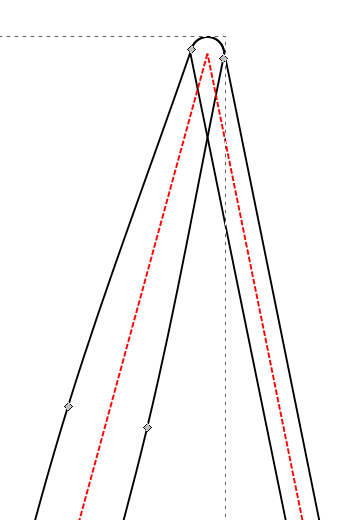
\includegraphics[height=5cm]{images/stroke_construction.png}
	\caption{Anatomy of continuous \texttt{CurvedStroke}s. Image shows clean combination of two strokes. Stroke outlines in black, with no fill applied to aid visualisation. Red dashed lines represent construction curves, from which the black outlines are derived through curve offsetting. Grey control points allow the length of each black outline path allow the stroke thickness to varied over its length (a slight taper is shown here on the leftmost stroke).}\label{stroke_construction}
\end{figure}

\FloatBarrier
\subsubsection{Discrete Strokes}

\texttt{Stipples} are much simpler to model, in that each stroke consists of two rounded end caps joined by straight lines.
However, this simple design allows for flexibility of styles - both head and tail radius is User-configurable, along with stroke length.
Currently, the System is implemented such that all stipples have the same shape/size, however the System is easy to extend to allow different variations of stipple strokes throughout the image.

\begin{figure}[h!]
	\centering
	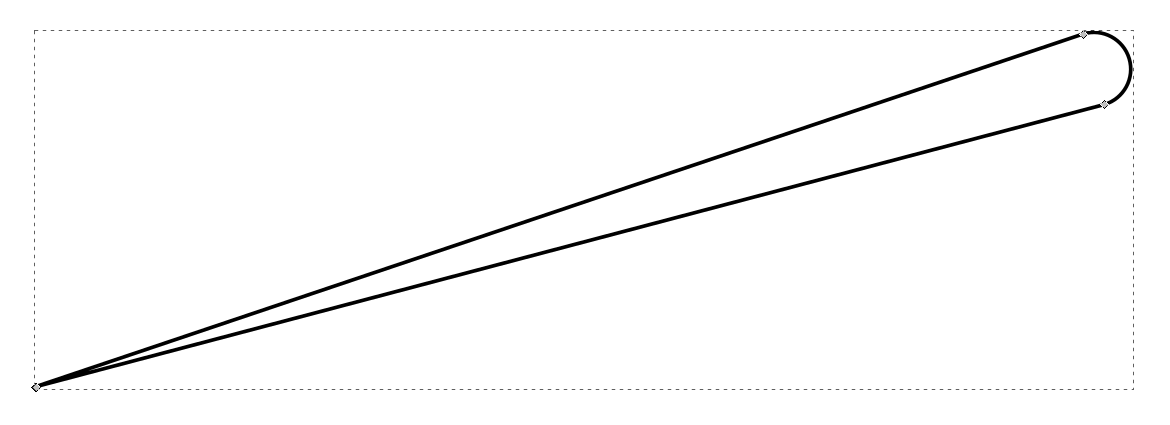
\includegraphics[height=5cm]{images/stipple_construction.png}
	\caption{Anatomy of a discrete \texttt{DirectionalStippleStroke}. Stroke outline in black, with no fill applied to aid visualisation. The radius of the ``tail'' end is set much smaller than the ``head'', to give a severe tapering style.}\label{stroke_construction}
\end{figure}

Talk about clipping.

\FloatBarrier
\section{Demonstration}
% - UI.
% - Sample render.
% - Performance.
